In our second example, we will use the built-in
\texttt{PoliticalDemocracy} dataset. This is a dataset that has been
used by Bollen in his 1989 book on structural equation modeling (and
elsewhere). To learn more about the dataset, see its help page and the
references therein.

The figure below contains a graphical representation of the model that
we want to fit.

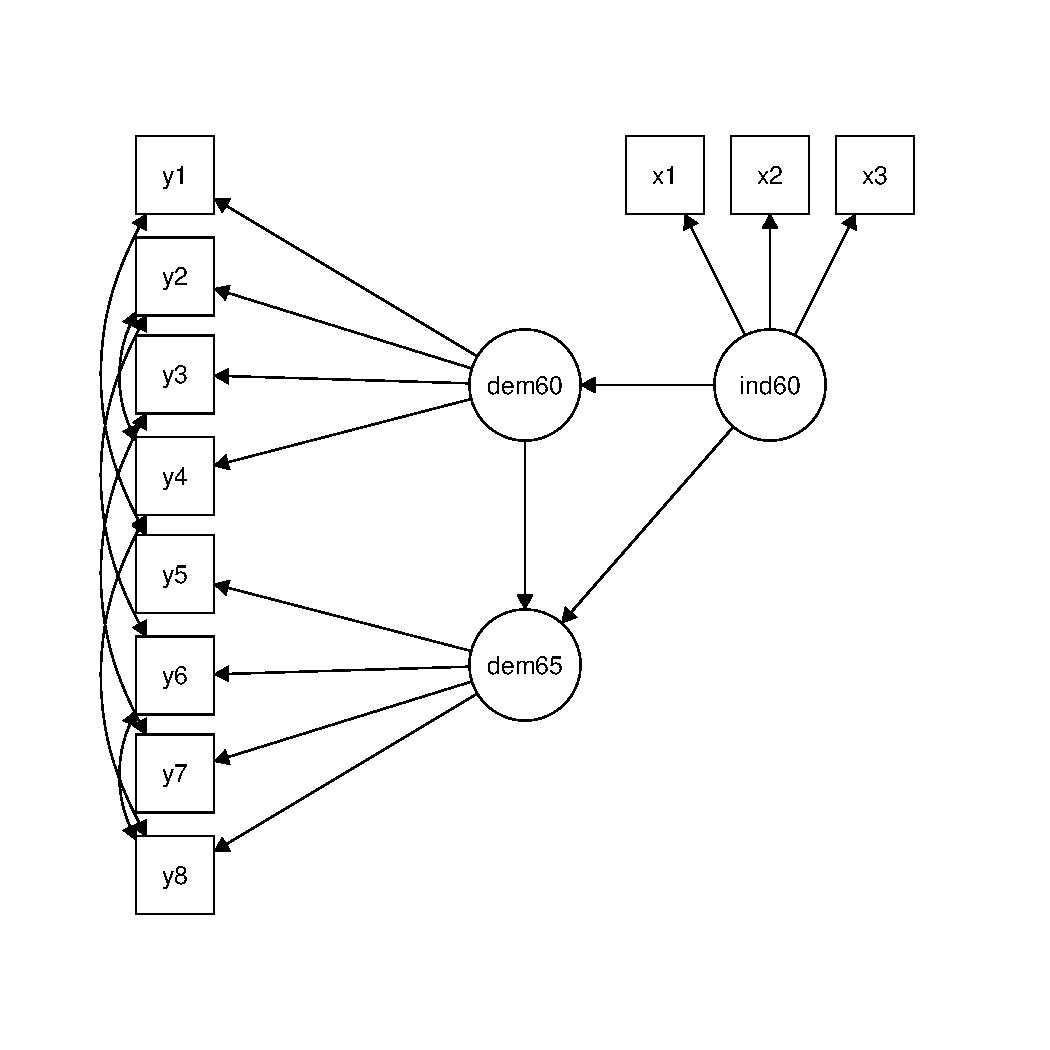
\includegraphics{figure/sem-1.pdf}

The corresponding lavaan syntax for specifying this model is as follows:

\begin{Shaded}
\begin{Highlighting}[]
\NormalTok{model }\OtherTok{\textless{}{-}} \StringTok{\textquotesingle{}}
\StringTok{  \# measurement model}
\StringTok{    ind60 =\textasciitilde{} x1 + x2 + x3}
\StringTok{    dem60 =\textasciitilde{} y1 + y2 + y3 + y4}
\StringTok{    dem65 =\textasciitilde{} y5 + y6 + y7 + y8}
\StringTok{  \# regressions}
\StringTok{    dem60 \textasciitilde{} ind60}
\StringTok{    dem65 \textasciitilde{} ind60 + dem60}
\StringTok{  \# residual correlations}
\StringTok{    y1 \textasciitilde{}\textasciitilde{} y5}
\StringTok{    y2 \textasciitilde{}\textasciitilde{} y4 + y6}
\StringTok{    y3 \textasciitilde{}\textasciitilde{} y7}
\StringTok{    y4 \textasciitilde{}\textasciitilde{} y8}
\StringTok{    y6 \textasciitilde{}\textasciitilde{} y8}
\StringTok{\textquotesingle{}}
\end{Highlighting}
\end{Shaded}

In this example, we use three different formula types: latent variabele
definitions (using the \texttt{=\textasciitilde{}} operator), regression
formulas (using the \texttt{\textasciitilde{}} operator), and
(co)variance formulas (using the
\texttt{\textasciitilde{}\textasciitilde{}} operator). The regression
formulas are similar to ordinary formulas in R. The (co)variance
formulas typically have the following form:

\begin{verbatim}
variable ~~ variable
\end{verbatim}

The variables can be either observed or latent variables. If the two
variable names are the same, the expression refers to the variance (or
residual variance) of that variable. If the two variable names are
different, the expression refers to the (residual) covariance among
these two variables. The lavaan package automatically makes the
distinction between variances and residual variances.

In our example, the expression
\texttt{y1\ \textasciitilde{}\textasciitilde{}\ y5} allows the residual
variances of the two observed variables to be correlated. This is
sometimes done if it is believed that the two variables have something
in common that is not captured by the latent variables. In this case,
the two variables refer to identical scores, but measured in two
different years (1960 and 1965, respectively). Note that the two
expressions \texttt{y2\ \textasciitilde{}\textasciitilde{}\ y4} and
\texttt{y2\ \textasciitilde{}\textasciitilde{}\ y6}, can be combined
into the expression
\texttt{y2\ \textasciitilde{}\textasciitilde{}~y4\ +\ y6}, because the
variable on the left of the \texttt{\textasciitilde{}\textasciitilde{}}
operator (\texttt{y2}) is the same. This is just a shorthand notation.

We enter the model syntax as follows:

\begin{Shaded}
\begin{Highlighting}[]
\NormalTok{model }\OtherTok{\textless{}{-}} \StringTok{\textquotesingle{}}
\StringTok{  \# measurement model}
\StringTok{    ind60 =\textasciitilde{} x1 + x2 + x3}
\StringTok{    dem60 =\textasciitilde{} y1 + y2 + y3 + y4}
\StringTok{    dem65 =\textasciitilde{} y5 + y6 + y7 + y8}
\StringTok{  \# regressions}
\StringTok{    dem60 \textasciitilde{} ind60}
\StringTok{    dem65 \textasciitilde{} ind60 + dem60}
\StringTok{  \# residual correlations}
\StringTok{    y1 \textasciitilde{}\textasciitilde{} y5}
\StringTok{    y2 \textasciitilde{}\textasciitilde{} y4 + y6}
\StringTok{    y3 \textasciitilde{}\textasciitilde{} y7}
\StringTok{    y4 \textasciitilde{}\textasciitilde{} y8}
\StringTok{    y6 \textasciitilde{}\textasciitilde{} y8}
\StringTok{\textquotesingle{}}
\end{Highlighting}
\end{Shaded}

To fit the model and see the results we can type:

\begin{Shaded}
\begin{Highlighting}[]
\NormalTok{fit }\OtherTok{\textless{}{-}} \FunctionTok{sem}\NormalTok{(model, }\AttributeTok{data =}\NormalTok{ PoliticalDemocracy)}
\FunctionTok{summary}\NormalTok{(fit, }\AttributeTok{standardized =} \ConstantTok{TRUE}\NormalTok{)}
\end{Highlighting}
\end{Shaded}

\begin{verbatim}
lavaan 0.6-11 ended normally after 68 iterations

  Estimator                                         ML
  Optimization method                           NLMINB
  Number of model parameters                        31
                                                      
  Number of observations                            75
                                                      
Model Test User Model:
                                                      
  Test statistic                                38.125
  Degrees of freedom                                35
  P-value (Chi-square)                           0.329

Parameter Estimates:

  Standard errors                             Standard
  Information                                 Expected
  Information saturated (h1) model          Structured

Latent Variables:
                   Estimate  Std.Err  z-value  P(>|z|)   Std.lv  Std.all
  ind60 =~                                                              
    x1                1.000                               0.670    0.920
    x2                2.180    0.139   15.742    0.000    1.460    0.973
    x3                1.819    0.152   11.967    0.000    1.218    0.872
  dem60 =~                                                              
    y1                1.000                               2.223    0.850
    y2                1.257    0.182    6.889    0.000    2.794    0.717
    y3                1.058    0.151    6.987    0.000    2.351    0.722
    y4                1.265    0.145    8.722    0.000    2.812    0.846
  dem65 =~                                                              
    y5                1.000                               2.103    0.808
    y6                1.186    0.169    7.024    0.000    2.493    0.746
    y7                1.280    0.160    8.002    0.000    2.691    0.824
    y8                1.266    0.158    8.007    0.000    2.662    0.828

Regressions:
                   Estimate  Std.Err  z-value  P(>|z|)   Std.lv  Std.all
  dem60 ~                                                               
    ind60             1.483    0.399    3.715    0.000    0.447    0.447
  dem65 ~                                                               
    ind60             0.572    0.221    2.586    0.010    0.182    0.182
    dem60             0.837    0.098    8.514    0.000    0.885    0.885

Covariances:
                   Estimate  Std.Err  z-value  P(>|z|)   Std.lv  Std.all
 .y1 ~~                                                                 
   .y5                0.624    0.358    1.741    0.082    0.624    0.296
 .y2 ~~                                                                 
   .y4                1.313    0.702    1.871    0.061    1.313    0.273
   .y6                2.153    0.734    2.934    0.003    2.153    0.356
 .y3 ~~                                                                 
   .y7                0.795    0.608    1.308    0.191    0.795    0.191
 .y4 ~~                                                                 
   .y8                0.348    0.442    0.787    0.431    0.348    0.109
 .y6 ~~                                                                 
   .y8                1.356    0.568    2.386    0.017    1.356    0.338

Variances:
                   Estimate  Std.Err  z-value  P(>|z|)   Std.lv  Std.all
   .x1                0.082    0.019    4.184    0.000    0.082    0.154
   .x2                0.120    0.070    1.718    0.086    0.120    0.053
   .x3                0.467    0.090    5.177    0.000    0.467    0.239
   .y1                1.891    0.444    4.256    0.000    1.891    0.277
   .y2                7.373    1.374    5.366    0.000    7.373    0.486
   .y3                5.067    0.952    5.324    0.000    5.067    0.478
   .y4                3.148    0.739    4.261    0.000    3.148    0.285
   .y5                2.351    0.480    4.895    0.000    2.351    0.347
   .y6                4.954    0.914    5.419    0.000    4.954    0.443
   .y7                3.431    0.713    4.814    0.000    3.431    0.322
   .y8                3.254    0.695    4.685    0.000    3.254    0.315
    ind60             0.448    0.087    5.173    0.000    1.000    1.000
   .dem60             3.956    0.921    4.295    0.000    0.800    0.800
   .dem65             0.172    0.215    0.803    0.422    0.039    0.039
\end{verbatim}

The function \texttt{sem()} is very similar to the function
\texttt{cfa()}. In fact, the two functions are currently almost
identical, but this may change in the future. In the \texttt{summary()}
function, we omitted the \texttt{fit.measures\ =\ TRUE} argument.
Therefore, you only get the basic chi-square test statistic. The
argument \texttt{standardized\ =\ TRUE} augments the output with
standardized parameter values. Two extra columns of standardized
parameter values are printed. In the first column (labeled
\texttt{Std.lv}), only the latent variables are standardized. In the
second column (labeled \texttt{Std.all}), both latent and observed
variables are standardized. The latter is often called the `completely
standardized solution'.

The complete code to specify and fit this model is printed again below:

\begin{Shaded}
\begin{Highlighting}[]
\FunctionTok{library}\NormalTok{(lavaan) }\CommentTok{\# only needed once per session}
\NormalTok{model }\OtherTok{\textless{}{-}} \StringTok{\textquotesingle{}}
\StringTok{  \# measurement model}
\StringTok{    ind60 =\textasciitilde{} x1 + x2 + x3}
\StringTok{    dem60 =\textasciitilde{} y1 + y2 + y3 + y4}
\StringTok{    dem65 =\textasciitilde{} y5 + y6 + y7 + y8}
\StringTok{  \# regressions}
\StringTok{    dem60 \textasciitilde{} ind60}
\StringTok{    dem65 \textasciitilde{} ind60 + dem60}
\StringTok{  \# residual correlations}
\StringTok{    y1 \textasciitilde{}\textasciitilde{} y5}
\StringTok{    y2 \textasciitilde{}\textasciitilde{} y4 + y6}
\StringTok{    y3 \textasciitilde{}\textasciitilde{} y7}
\StringTok{    y4 \textasciitilde{}\textasciitilde{} y8}
\StringTok{    y6 \textasciitilde{}\textasciitilde{} y8}
\StringTok{\textquotesingle{}}
\NormalTok{fit }\OtherTok{\textless{}{-}} \FunctionTok{sem}\NormalTok{(model, }\AttributeTok{data=}\NormalTok{PoliticalDemocracy)}
\FunctionTok{summary}\NormalTok{(fit, }\AttributeTok{standardized=}\ConstantTok{TRUE}\NormalTok{)}
\end{Highlighting}
\end{Shaded}
